\chapter{Installation de virt-manager}
\section{Installation côté serveur}
Cette partie est facile, un simple apt-get install suffit. Nous installons le paquet qui communique avec Xen et remonte les informations au client virt-manager.
\begin{lstlisting}
apt-get install libvirt-bin
\end{lstlisting} 
Du coté de Xen, nous devons vérifier qu’il peut communiquer avec libvirt.

Libvirt accède aux données de Xen via un socket unix. La configuration consiste à activer cette option dans Xen et à relancer les services.
Nous éviterons ainsi l’erreur libvirtError: internal error failed to connect to xend dont on trouve peu d’explication sur le net.

On édite le fichier de configuration xen
\begin{lstlisting} 
nano /etc/xen/xend-config.sxp
\end{lstlisting}
 on active la ligne suivante
\begin{lstlisting} 
(xend-unix-server yes)
\end{lstlisting}
 Enfin on relance le service xen avec /etc/init.d/xend restart

\section{Installation côté client}
Pour gérer nos serveurs, nous installons virt-manager avec la commande suivante:
\begin{lstlisting} 
apt-get install virt-manager
\end{lstlisting}
\chapter{Création d'hôtes virtualisée avec virt-manager}


1)Pour commencer on démmarre virt-manager, puis on lance le gestionnaire de machines virtuelles à partir du menu en cliquant sur l'icone en forme de pc.



3) La fenêtre du gestionnaire de machine virtuelle nous autorise à en créer de nouvelles.
On clique sur création de nouvelle machine virtuelle pour faire apparaître l'assistant qui va nous aider pour élaborer notre hôte.
L'assistant décompose la création en cinq étapes:
-La localisation et la configuration des supports d'installation
-La configuration de la mémoire et les options de CPU
-La configuration du stockage de l'invité
-La configuration réseau, l'architecture, et d'autres paramètres matériels

Le processus de création d'hôte commence avec la selection d'un nom et le type d'installation.
-------------------------------
ON MET UNE IMAGE POUR MONTRER
-------------------------------
-Local install media(ISO image or CDROM)
Cette méthode utilise un CD-ROM,DVD ou une image iso.

-Network install
Cette méthode utilise le réseau pour installer le système d'exploitation.

-Import existing disk image
Cette méthode nous permet de créer un nouvelle hôte et d'y importer une image disque.

La prochaine étape consiste à configurer l'installation.
On configure le type de système d'exploitation et sa version qui sera installé, cela dépend de la méthode d'installation que l'on a choisie.
-----------------------------------------------
ON MET UNE IMAGE
-----------------------------------------------
-----------------------------------------------
ON MET UNE IMAGE
-----------------------------------------------

Configuration du CPU et de la mémoire
La prochaine étape consiste à configurer le nombre de CPU et la quantité de mémoire à allouer à la machine virtuelle. L'assistant indique le nombre de processeurs et la quantité de mémoire que l'on peut lui allouer.
-------------------------------------------------------
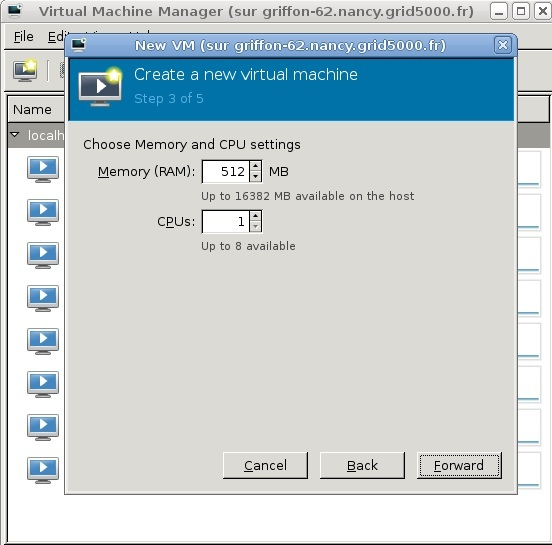
\includegraphics{images/cpu.jpg}
Configuration de l'espace de stockage
-------------------------------------------------------
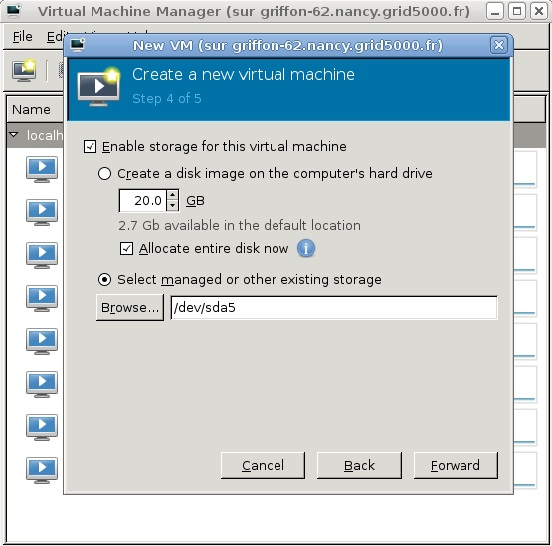
\includegraphics{images/Storage.jpg}
-------------------------------------------------------
 Si l'on a choisi d'importer une image de disque existante au cours de la première étape, virt-manager va sauter cette étape.
On doit attribuer un espace suffisant pour notre machine virtuelle et toutes les applications que l'hôte a besoin.

Configuration finale
On vérifie les paramètres de la machine virtuelle et on clique sur Terminer lorsqu'on est satisfait, cela permettra de créer l'hôte avec les paramètres réseau par défaut, le type de virtualisation, et l'architecture.
